\newcommand{\numsides}{oneside}    % Un côté pour la version électronique 
%\renewcommand{\numsides}{twoside} % Décommenter -> version imprimée (2 côtés)

\documentclass[titlepage,\numsides,openright,letterpaper,12pt]{book}
\usepackage{entete,commandes} % Load les packages et définit des commandes.

%=============================================================================%

% On crée des bools qui sont False par défaut.
\newtoggle{AuteureFemme}
\newtoggle{MemoirePasThese}
\newtoggle{useCustomFonts}

% Switchboard, l'endroit ou on ajuste les toggles.
% Décommenté -> True; commenté -> False
%
%\toggletrue{AuteureFemme}     % Décommenter si l'auteur est une femme.
%\toggletrue{MemoirePasThese}  % Décommenter dans le cas d'un mémoire.
\toggletrue{useCustomFonts}   % Fonts différents, voir switchboard.tex.

% On cache le code exécuté dans ce fichier parce qu'il est laid et impertinent.
\begin{comment}
\end{comment}

\makeatletter   % Permet d'accèder aux variables @

%=============================================================================%

    \iftoggle{useCustomFonts}
    {   
        % Deux prochaines lignes -> Pagella et Mathpazo
        \usepackage{mathpazo} % utilise Palatino pour les mathématiques (mettre en premier)
        \usepackage{tgpagella} % utilise la police TeX Gyre Pagella

        % Deux prochaines lignes -> New Century et Fourier
        %\usepackage{newcent}
        %\usepackage{fouriernc}
    }
    {}

%=============================================================================%
    
    \iftoggle{AuteureFemme}
    { \newcommand{\monsieurMadame}{Mme.} }    
    { \newcommand{\monsieurMadame}{M.} }

%=============================================================================%

    \iftoggle{MemoirePasThese}
    {   % Si c'est un mémoire
        \newcommand{\documentPresente}{Mémoire présenté}
        \newcommand{\leDocument}{le mémoire}
        \newcommand{\leGrade}{maître ès science (M.Sc.)}
    }
    {   % Si c'est une thèse
        \newcommand{\documentPresente}{Thèse présentée}
        \newcommand{\leDocument}{la thèse}
        \newcommand{\leGrade}{docteur ès science (Ph.D.)}
    }

%=============================================================================%
    
    % Gestion de la version électronmique vs celle imprimée.
    \newtoggle{oneside}     % Truc pour avoir un else à \if@twoside
    \toggletrue{oneside}
    \if@twoside
        \togglefalse{oneside}
    \fi

    \iftoggle{oneside}
    {   % S'il y a un côté, on fait la version électronique.
        \geometry{letterpaper, lmargin=1.25in, rmargin=1.25in,
                  tmargin=1.5in, bmargin=1.0in}
        % Prochaines trois lignes enlève l'entête
        \renewcommand{\chaptermark}[1]
            {\markboth{{\thechapter. #1}}{}}
        \renewcommand{\sectionmark}[1]{}
        % On n'affiche pas les DOI dans la biblio -> Plus propre
        \bibliographystyle{nature-fr}
        %\bibliographystyle{unsrt-fr} % unsrt partiellement traduit. Préférer nature.
    }
    {   % S'il y a deux côtés, on fait la version imprimée!

        % On enlève la numérotation des pages vides
        \let\origdoublepage\cleardoublepage
        \newcommand{\clearemptydoublepage}{%
            \clearpage
            {\pagestyle{empty}\origdoublepage}%
            }
        \let\cleardoublepage\clearemptydoublepage
 
        % Chapitre à la page de droite avec une page gauche blanche
        \let\stdchapter\chapter
        \renewcommand*\chapter{%
              \@ifstar{\starchapter}{\@dblarg\nostarchapter}}
              \newcommand*\starchapter[1]{\clearpage\null\thispagestyle{empty}\stdchapter*{#1}}
              \def\nostarchapter[#1]#2{\clearpage\null\thispagestyle{empty}\stdchapter[{#1}]{#2}}

        % On utilise un fontsize plus petit pour un livre (10pt vs 12pt).
        \let\small\relax
        \let\footnotesize\relax
        \let\scriptsize\relax
        \let\tiny\relax
        \let\large\relax
        \let\Large\relax
        \let\LARGE\relax
        \let\huge\relax
        \let\Huge\relax
        \input{size10.clo}

        % Les hyperliens n'ont pas desoins d'être colorés
        \hypersetup{hidelinks}
        % On affiche les DOI dans la biblio -> Pratique en version imprimée
        \bibliographystyle{nature-fr-showdoi}
    }

%=============================================================================%

\makeatother    % Plus d'accès aux variables @


%=============================================================================%

\begin{document}
\title{Titre descriptif, pertinent et évocateur} % Pour la page de titre/jury.
\author{ Auteur(e) }  % Idem
\date{\today}       % Idem

%=============================================================================%



%=============================================================================%
% Titre
\begin{comment}
\end{comment}
\makeatletter   % Permet d'accèder aux variables @

\thispagestyle{empty}  % Page blanche avec formattage manuel
\pagenumbering{gobble} % Aucune numérotation, sinon hypperref bug
\vglue 2cm
\begin{center}
    \doublespacing{
    {\LARGE \@title}\\
    \vspace{2.0cm}
    par\\
    \vspace{2.0cm}
    {\large \@author}
    \vspace{2.0cm}\\
    \documentPresente\ au département de physique\\
    en vue de l'obtention du grade de \leGrade
    \vfill
    FACULTÉ des SCIENCES\\
    \Organisation\vspace{1.0cm}\\
    \Location, \@date  % La date sera celle de la compilation
    }
\end{center}

\makeatother    % Plus d'accès aux variables @


\frontmatter % Pagination de préambule

% Jury
\begin{comment}
\end{comment}
\makeatletter   % Permet d'accèder aux variables @

% Next two lines force a linebreak in ebook versions
\chapter*{}
\vspace{-4.7cm}

\thispagestyle{empty}

\begin{center}
    \vglue 2cm
    Le \underline{\hspace{5cm}}\\ 
    %Le \@date % Lorsque le document sera accepté!
    \vspace{2cm}
    \scalebox{1} % Empêche le retour à la ligne si le nom est trop long.
    {\it le jury a accepté \leDocument\ de \monsieurMadame~\@author~dans sa version finale.} 
    
    \vspace{2cm}
    Membres du jury\\
    \vspace{2cm}

    Professeur \underline{\hspace{2.5cm}}\\
    Directeur de recherche\\
    Département de physique\\
    \vspace{2cm}
    
    Professeur \underline{\hspace{2.5cm}}\\
    Membre interne\\
    Département de physique\\
    \vspace{2cm}

    Professeur \underline{\hspace{2.5cm}}\\
    Président rapporteur\\
    Département de physique\\
    \vspace{2cm}
\end{center}

%\clearpage

\makeatother    % Plus d'accès aux variables @


% Dédicace
\begin{comment}
\end{comment}

\chapter*{}
\vspace{-10pt}
\begin{flushright}
    À \underline{\hspace{4cm}}
\end{flushright}

\thispagestyle{empty}

% Sommaire
\clearpage  % Mets le sommaire à la bonne page dans la TOC
\chapter*{Sommaire}
\addcontentsline{toc}{chapter}{Sommaire}
\begin{comment}
\end{comment}

\kant[1]


% Remerciements
\chapter*{Remerciements}
\begin{comment}
\end{comment}

\markboth{Remerciements}{Remerciements}
\kant[2-3] % Remplissage



% Tables des matières/Figures
{
    \setlength{\parskip}{0ex}
    \tableofcontents
    \listoffigures
    %\listoftables
}

%=============================================================================%

\mainmatter % Pagination standard
\onehalfspacing

%-----------------------------------------------------------------------------%

\chapter{Introduction}
\begin{comment}
\end{comment}

\Introduction   % Chapitre qui ne sera pas numéroté si IntroConcluSansNombre est Vrai

%-----------------------------------------------------------------------------%

\kant[4-7] % Remplissage


\chapter{Théorie}
\begin{comment}
\end{comment}

\chapter{Théorie}

%-----------------------------------------------------------------------------%

% Ce qui suit n'est que du remplissage avec un petit exemple de ref/eqref
\section{Section}
\subsection{Exemple math \label{sec:newton}}

Newton a reçu -- ou pas -- une pomme sur la tête avant de déterminer, dans \cite{newton1687philosophiae}, que
\begin{align}
    \label{eq:newton}
    \vec F=m \vec a,
\end{align}
son équation la plus célèbre. Comme on le voit donc à l'équation~\eqref{eq:newton} de la section~\ref{sec:newton}, la force est proportionnelle à l'accélération.

On peut aussi exprimer la mécanique sous la forme lagrangienne. Pour des coordonnées généralisées $q$ et leur dérivées $\dot q$, le lagrangien est alors

\begin{align}
    \label{eq:lagrangien}
    L(q, \dot q, t) = T - V
\end{align}

et les équations du mouvement dérivent des équations de Lagrange 

\begin{align}
    \label{eq:equations_lagrange}
    \frac{\partial L}{\partial q} - \frac{\mathrm{d}}{\mathrm{d}t}\frac{\partial L}{\partial \dot q} = 0 \quad \forall q
    .   % Fin de la phase -> point
\end{align}

Ainsi, bien que ça ne soit pas évident de prime abord, les équations~\eqref{eq:newton} et~\eqref{eq:equations_lagrange} sont conceptuellement équivalentes!

\subsection{Exemple citation}
Citons aussi un vieil article \cite{andreev1964} et un autre \cite{robertson1929}. Maintenant citons les deux à la fois \cite{andreev1964, robertson1929}. Ensuite, citons plusieurs références avec un commentaire chacunes \cites[p.~1]{robertson1929}[chap.~2]{andreev1964}[\textsection 6]{newton1687philosophiae}. Finalement, citons les mêmes références, mais ne mettons des commentaires que lorsque nécessaire \cites{robertson1929}[chap.~2]{andreev1964}{newton1687philosophiae}.

\subsection{Parenthèses ajustables}
Voici des exemples d'utilisantion des paranthèses ajustables définies dans le package \emph{commandes}\footnote{Voici comment faire une note en bas de page. Voir le fichier \texttt{commandes.sty} pour des commandes personnalisées et personnalisables.}:
\begin{align}
    a&=\p{123}            \\
    a&=\p[]{123}          \\
    a&=\p[big]{123}       \\
    a&=\pc[Big]{123}      \\
    a&=\pc[bigg]{123}     \\
    a&=\pa[Bigg]{123}     \\
    a&=\pa[none]{123}     \\
    a&=\moy{\int t\dd t}  \\
    a&=\norm{\int t\dd t} \\
    a&=\abs[Bigg]{123}    \\
\end{align}

\subsection{Remplissage}
\kant[8-10]



\chapter{Résultats}
\begin{comment}
\end{comment}

\chapter{Résultats}

%-----------------------------------------------------------------------------%

\section{Exemple de graphique}

La figure~\ref{fig:phdcomics} est très drôle, sérieusement.

\begin{figure}[htb]
    \begin{center}
        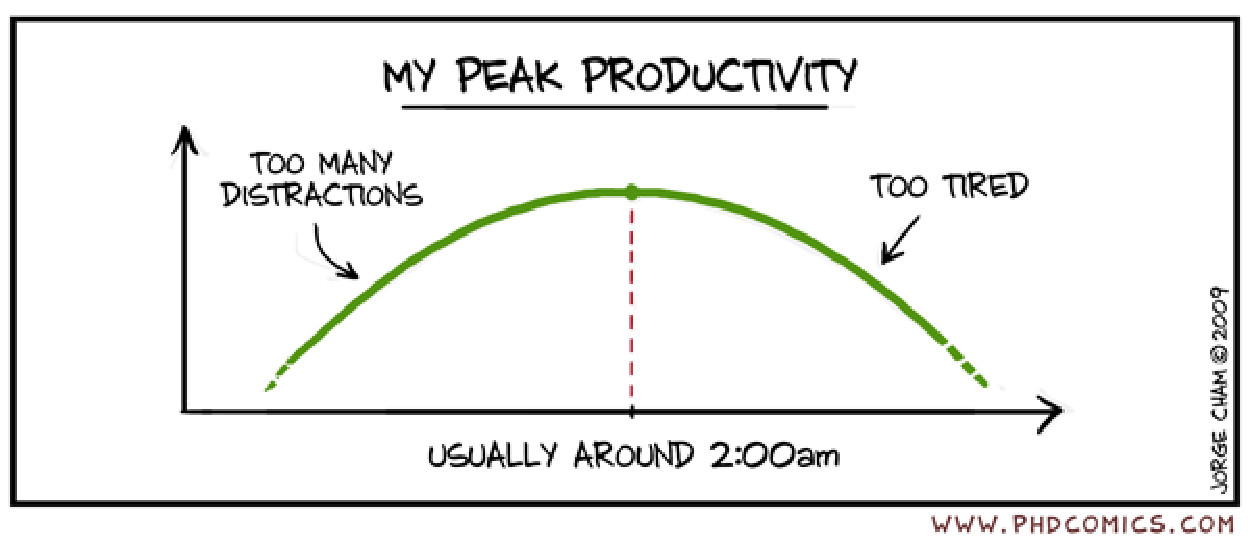
\includegraphics[width=0.8\columnwidth]{Figures/phd083109s.pdf} 
        \longcaption{Figure à la fois hilarante et véridique.}{Image tirée du webcomic "Piled Higher and Deeper" par Jorge Cham \href{www.phdcomics.com}{www.phdcomics.com}. Seule la première partie de ce long caption sera dans la table des figures.}
        \label{fig:phdcomics}
    \end{center}
\end{figure}

\section{Remplissage}
\kant[11-14]


\chapter{Conclusion}
\begin{comment}
\end{comment}

\Conclusion % Chapitre qui ne sera pas numéroté si IntroConcluSansNombre est Vrai

%-----------------------------------------------------------------------------%

\kant[15-17]


%-----------------------------------------------------------------------------%

\singlespacing

\appendix
\renewcommand\chapterstring{Annexe}
\chapter{Matériel Supplémentaire}
\begin{comment}
\end{comment}

\kant[18-20]


%=============================================================================%

% Voir switchboard.tex pour le bibliographystyle selon le type de document.
\bibliography{memoire}        % Le fichier de bibliographie est memoire.bib.

\end{document}
